\chapter{Theory}\todo{Lad det her med opdelingen simre.}
This thesis takes the perspective of viewing all eye information sources as well as their encodings as signals. This perspective is exceptionally useful when analysing uncertainty in a complex system composed of multiple information sources and with multiple goals. Additionally, it allows us to treat the objective of information obfuscation abstractly and thereby consider its use across multiple different applications. It turns out that any information extraction process can be defined in terms of just its ability to preserve the original information and be robust to noise. As a result, obfuscation methods are defined by competing goals of signal preservation for one information source (gaze) and signal degradation for another, e.g. the iris pattern. This chapter introduces and discusses the necessary prerequisites assuming a reader with knowledge of fundamental probability theory. The next chapter uses the presented theory to describe the abstract model and its implications.


%The proposed methodology and experiments rely on interpretations of eye tracking and iris recognition as communication systems of discrete signals. This requires a fundamental knowledge of information theory and signal processing which concern how uncertainty propagates and ...

%As presented in the overview, attributes such as gaze direction and personal identity can be represented as properties. These signals are encoded as physical properties which are transmitted through the medium of photons reflecting off of the eye onto a photosensitive camera sensor. This transmission creates an image, which is then processed further to ultimately decode the original properties. This is fundamentally similar to how a text message might be encoded and transmitted over a radio network to enable long distance communication.

%Information theory provides a number of tools for analysing such information transmission scenarios.
\section{Signals and information}
\begin{figure}
    \centering
    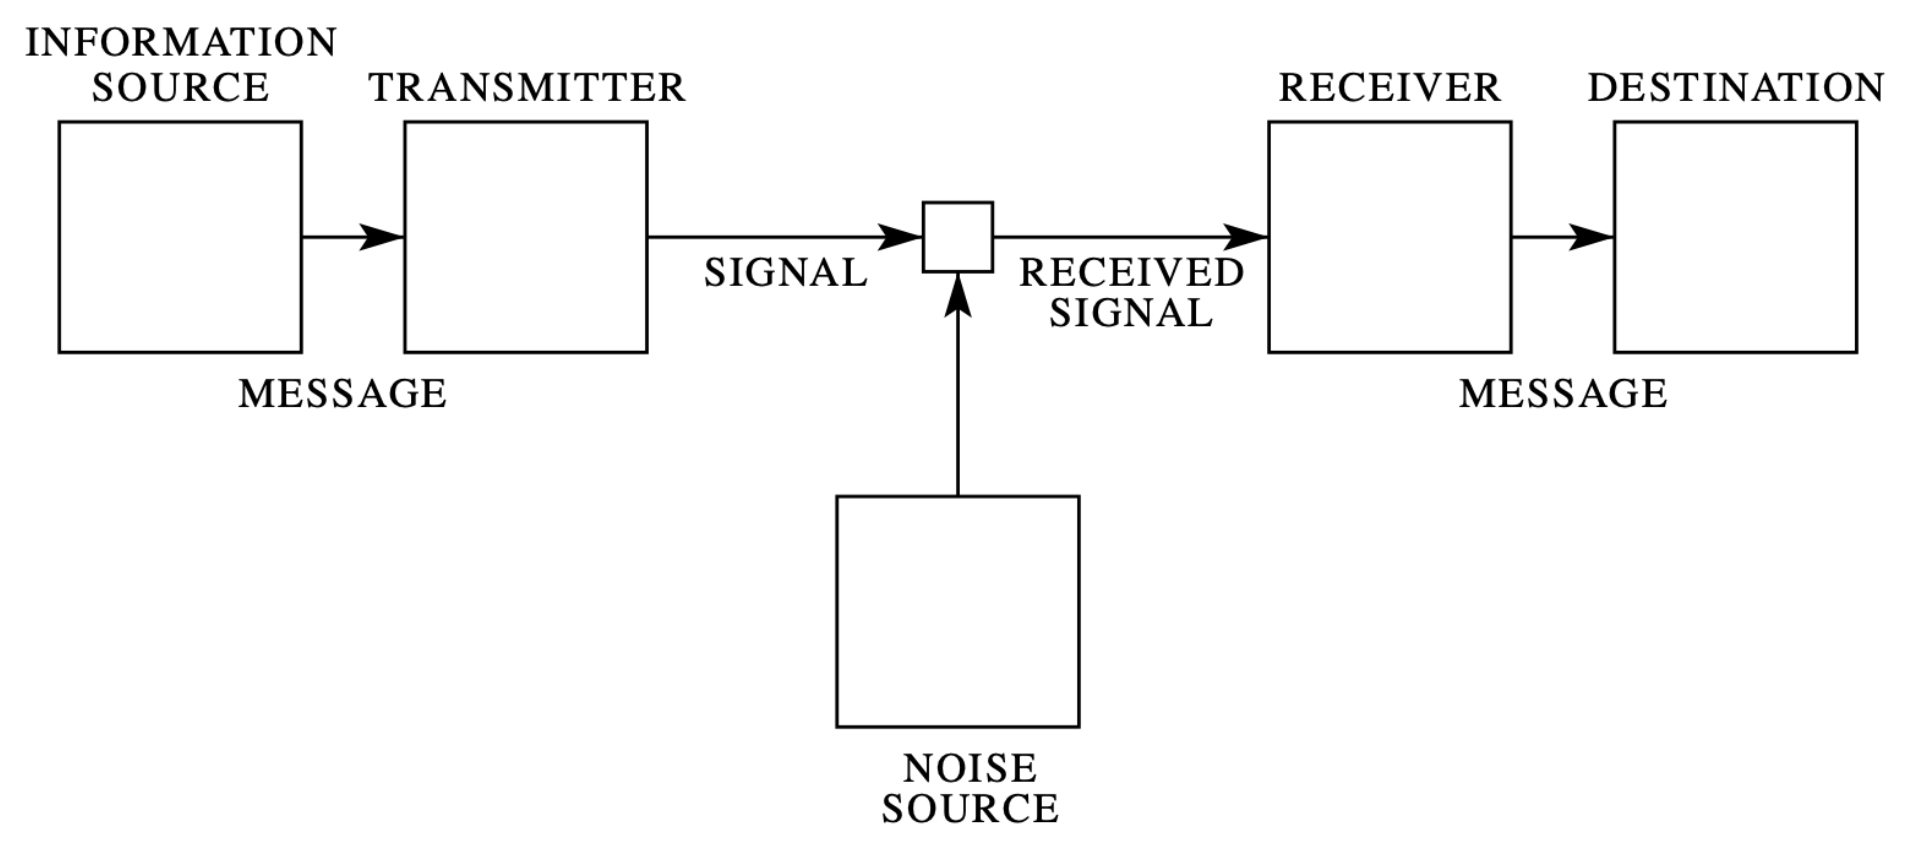
\includegraphics[width=0.8\textwidth]{figures/theory/comm-model.png}
    \caption{Diagram of communication system as depicted in \textit{A Mathematical Theory of Communication} \parencite{shannon1948mathematical}.}
    \label{fig:comm-model}
\end{figure}

\textit{Signal} is a rather vague term that is typically used to describe data that is transmitted over some medium and that contains \textit{meaningful information}. In this thesis, we use signal to denote any meaningful information that has been encoded by an arbitrary process. For example, the physical position and rotation of the eye is an encoding of several properties including point of regard. Information theory is a theoretical framework introduced by Claude Shannon for precisely measuring uncertainty in communication systems (REF). The signals of interest in case of eye-tracking and obfuscation methods are either images or time-based signals such as gaze or eye-feature parameters. These signals are only observed in discrete intervals defining units of time, space, or both. We therefore only consider the discrete parts of information theory. 

As shown in \cref{fig:comm-model}, a communication system consists of an information source that is transmitted as a signal over a channel and then decoded back into its original representation. This basic diagram can be applied to many kinds of situations including error handling, compression, and, as proposed in this thesis, eye information obfuscation.


Information theory defines entropy as a measure of uncertainty. It is a logarithmic function of the randomness of the transmitted signal. 
The base measure is entropy, denoted $H$ which defines the optimal average encoding length of symbols $x_i$ drawn from a discrete distribution $X$ defined by
\todo{Alt herunder skal revideres med flere detaljer + mere historiefortælling}
\begin{definition}[Shannon entropy]
The Shannon entropy is the expectation of the self information $I(X)$ of each outcome of $X$:
\begin{equation}
    H(x) = \mathbb{E}[h_X(X)] = - \sum_i p_i\log p_i
\end{equation}
\end{definition}

with results in the units of bits. Different bases may be used for alternate units. A uniformly distributed discrete random variable has an entropy of $\log{N}$ which is maximal for its number of states. In terms of iris recognition, the entropy of code symbols (bits are typically used) can be used to calculate the expected amount of information present in the entire signal. For example, Daugman calculated the expected iris code entropy by fitting a binomial distribution to the iris code distance comparisons, which revealed an approximate 250 bits of information between codes (REF). This entropy only accounts for the information content in the final codes and thus does not account for noise added during the encoding and processing steps. 

Analogous to conditional probability, the notion of conditional entropy signifies the entropy of a signal given knowledge of another. In \cref{fig:comm-model}, the conditional entropy can only originate from the noise source but in general, any number of signals may be combined in a channel and affect the conditional entropy. It can be defined in terms of the distributions of input and output signals $X$, $Y$.

\begin{definition}[Conditional entropy]
For random variables $X$, $Y$, the conditional entropy $H(Y|X)$ is defined by:
\begin{equation}
    H(Y|X) = \sum_{x\in\mathcal{X}, y\in\mathcal{Y}} p(x, y)\log\frac{p(x, y)}{p(x)}
\end{equation}.
\end{definition}

When a signal is transmitted over a channel, the mutual information defines the amount of uncertainty in the channel output that originates from the original signal. This measure is thus limited by the entropy of the source signal.

\begin{definition}[Mutual information]
The Shannon entropy is the expectation of the self information $I(X)$ of each outcome of $X$:
\begin{equation}
    I(Y;X) = \sum_{x\in\mathcal{X}, y\in\mathcal{Y}} p(x, y)\log\frac{p(x, y)}{p(x)p(y)}
\end{equation}
\end{definition}

The entropy of input and output signals $X$, $Y$ is related by how much information is shared between them (mutual information) and how much is introduced by the channel (conditional information). \cref{fig:entropy-comp} visualises this relationship which is written as
%The signal entropy over a channel can be decomposed into exactly the entropy carried over from the original signal (mutual information) and the noise introduced by the channel itself (conditional information) as shown visually in \cref{fig:entropy-comp}. This is encoded in the following relationship
\begin{align}\label{eq:entropy-law}
    H(X) = I(X;Y)+H(X|Y).
\end{align}

This is easily derived from the definitions of mutual information and conditional information
\begin{align*}
    I(X;Y)+H(X|Y) &= \sum_{x\in\mathcal{X}, y\in\mathcal{Y}} p(x, y)\log\frac{p(x,y)}{p(x)p(y)} + \left(-\sum_{x\in\mathcal{X}, y\in\mathcal{Y}} p(x, y)\log\frac{p(x,y)}{p(y)} \right) \\
    &= \sum_{x\in\mathcal{X}, y\in\mathcal{Y}} p(x,y)\left(\log{p(x,y)}-\log{p(x)}-\log{p(y)}-\log{p(x,y)}-\log{p(y)}\right)\\
    &= \sum_{x\in\mathcal{X}, y\in\mathcal{Y}} p(x,y)\log\frac{1}{p(x)}\\
    &= - \sum_{x\in\mathcal{X}} p(x)\log{p(x)}\\
    &= H(X).
\end{align*}

\begin{figure}
	\centering
	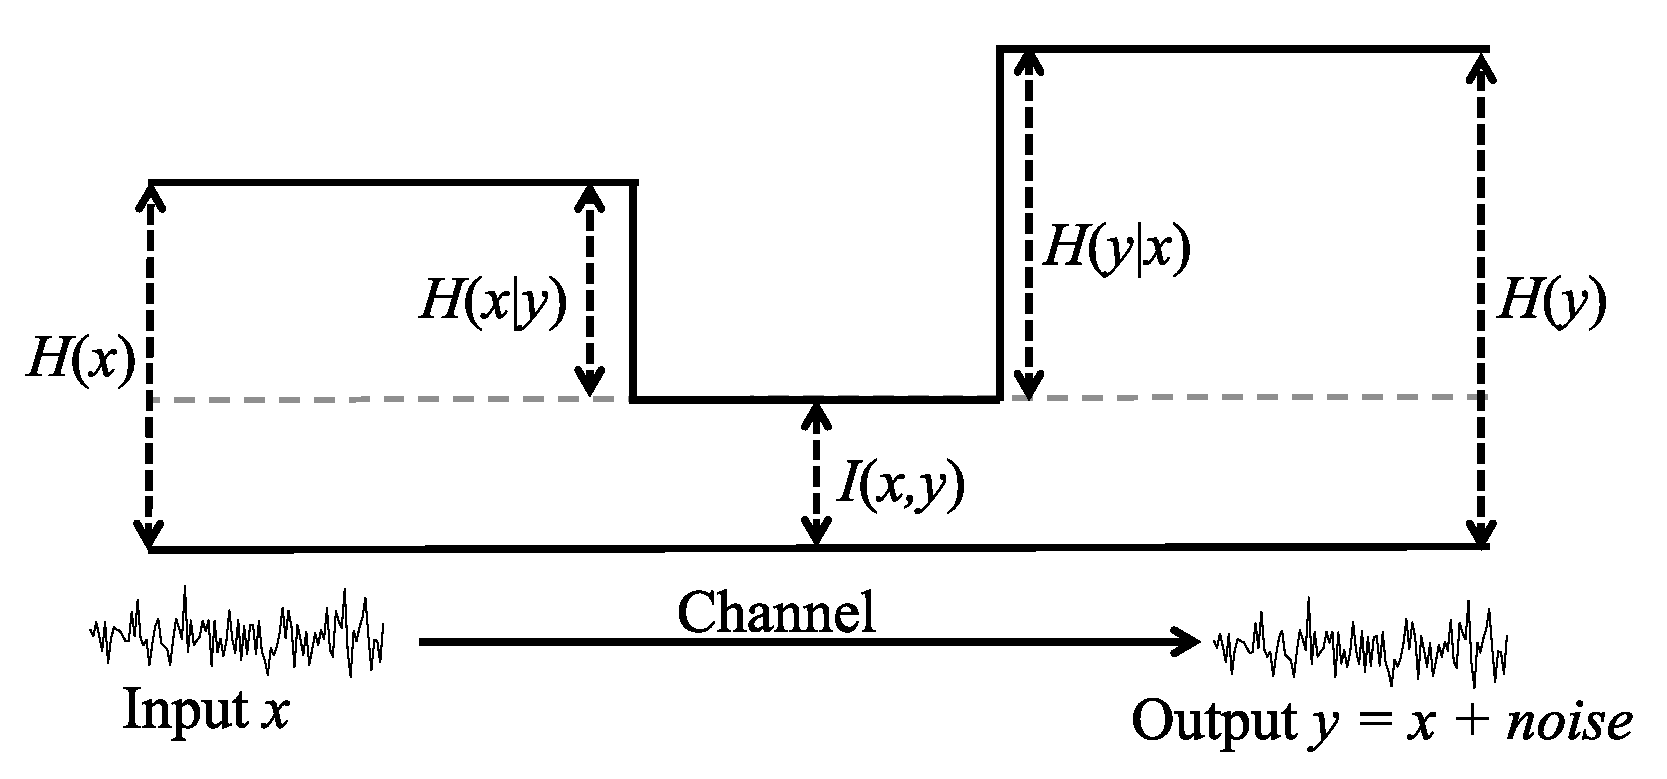
\includegraphics[width=0.8\textwidth]{figures/theory/entropy-comp}
	\caption{Hej}\label{fig:entropy-comp}
\end{figure}





%For iris obfuscation, the goal is to minimise $I(R_{iris}, Q_{iris})$ and maximise $I(R_{gaze}, Q_{gaze})$. Measuring these directly is again not possible as the $Q$ signals are not the measured signals. The only known information source is the image $I$ where the two signals have been combined into a single signal. However, because $H(Q_{gaze})$ should be very low, i.e. it represents an encoding of just two real values, the mutual information between the original and obfuscated images $I(I, I^*)$ can be used as a proxy to measure the level of obfuscation. Additionally, for any set of signals $X, Y, Z$ where $Z = f_z(Y)$ and $Y= f_z(X)$, then $I(Z; Y) \leq I(Z;X)$ (REF to proof). Thus, it is an upper bound for the mutual information which makes the results much more useful.

Finally, the notion of channel capacity is used to define the maximum mutual information of a channel for any input distribution. It is defined as
\begin{align}
    C = \max_{p_x} I(X, Y).
\end{align}
The channel capacity of specific obfuscation methods define strong upper limits on the amount of information that is able to pass. If an obfuscation method has capacity below the minimum requirement for differentiation of a population given the optimal distribution (uniform), it is impossible to accurately differentiate between all individuals. In practice, however, the image signal which is measured contains orders of magnitude more information, making such guarantees unlikely, at least for the methods presented in this paper. Instead, we use the measure to evaluate the relative obfuscation of information.

%%%%%%%%%%%%%%%%%%%
% Extra stuff - unlikely to get time to fix
%%%%%%%%%%%%%%%%%%%

%\subsection{Properties of mutual information}
%Mutual information can be generalised to multivariate cases. In ...

%\begin{definition}
%Given a set of $n$ random variables $X$, the mutual information between any subset $S\subset X$ is less than the mutual information of the whole set, i.e.
%\begin{equation}
%     I(S) \leq I(X)
%\end{equation}
%\end{definition}

%proof: By the definition of measures, the mutual information $I$ is always non-negative, i.e. $I > 0$. Since $I(X) = I(X^1, \dots, X^{n-1}) - I(xxx)$, $I(X^1, \dots, X^{n-1}) \leq I(X)$.

%%%%%%%%%%%%%%%%%%%

% \section{Information theory}
% Uncertainty is similar to electrical voltage in that it represents a relative difference between knowledge and the lack thereof. Information is a measure of change in uncertainty over time. In other words, a highly uncertain message will impart the receiver with a large amount of information on arrival. If the receiver already knows part of the message, they will be less uncertain of its contents and therefore receive less information on arrival. 

% Information theory is a mathematical field which defines a useful theoretical model for information along with a large body of work In essence, information theory uses the language of probability and measures to define and quantify uncertainty of the signals and transmission procedures.



% Information represents the gap between not knowing and knowing and is thus inherently relative. It is similar to electrical voltage in that 

% The fact that information is a measure of uncertainty might seem counter intuitive when it feels like information should be the lack of uncertainty. This is, not surprisingly, the result of a misunderstanding. Information is not the randomness itself, but instead represents the amount of uncertainty removed when a random variable is observed.

% \begin{definition}[Self information]
% \begin{equation}
%     h_x(x) = -log(p_x(x))
% \end{equation}
% \end{definition}

% \begin{definition}[Shannon entropy]
% The Shannon entropy is the expectation of the self information $I(X)$ of each outcome of $X$:
% \begin{equation}
%     H(x) = \mathbb{E}[h_X(X)] = - \sum_i p_i\log p_i
% \end{equation}
% \end{definition}

% \begin{definition}[Joint entropy]
% The Shannon entropy is the expectation of the self information $I(X)$ of each outcome of $X$:\todo{Detailed description - shorten notation and provide explanations}
% \begin{multline}
%     H(X^1, \dots, X^n) = -\mathbb{E}[h_X(X^1, \dots, X^n)] =\\ - \sum_{x^1\in\mathcal{X^1}} \dots \sum_{x^n\in\mathcal{X^n}} p_{X^1, \dots, X^n}(x^1, \dots, x^n)\log p_{X^1, \dots, X^n}(x^1, \dots, x^n)
% \end{multline}
% \end{definition}

% \begin{definition}[Conditional entropy]
% The Shannon entropy is the expectation of the self information $I(X)$ of each outcome of $X$:
% \begin{equation}
%     H(Y|X) = \sum_{x\in\mathcal{X}, y\in\mathcal{Y}} p(x, y)\log\frac{p(x, y)}{p(x)}
% \end{equation}
% \end{definition}

% \begin{definition}[Mutual information]
% The Shannon entropy is the expectation of the self information $I(X)$ of each outcome of $X$:
% \begin{equation}
%     I(Y;X) = \sum_{x\in\mathcal{X}, y\in\mathcal{Y}} p(x, y)\log\frac{p(x, y)}{p(x)p(y)}
% \end{equation}
% \end{definition}

% \begin{equation}
%     H(X) = H(X|Y) + I(X;Y)
% \end{equation}

% \begin{definition}[KL divergence]
% The Shannon entropy is the expectation of the self information $I(X)$ of each outcome of $X$:
% \begin{equation}
%     D_{KL}(P||Q) = \sum_{x\in\mathcal{X}}p(x)\log\frac{p(x)}{q(x)}
% \end{equation}
% \end{definition}

% \begin{align}
%     I(Y; X) = D_{KL}(p_{x,y}||p_x\times p_y)
% \end{align}

% \chapter{Information and signals}
% This chapter reviews the theoretical tools used for the modelling and analysing eye information in this thesis. It is an expanded version of the presentation in the article and reveals more details of how the theoretical parts connect and have directly inspired the solution proposals.



\section{Signal processing}
The field of signal processing generally concerns signals that are at least approximately continuous. The reason is that many real-world phenomena when measured resemble continuous functions. More specifically, signal processing concerns how to characterise and transform signals measured at discrete intervals using frequency analysis (REF?). It is widely used in computer vision.

The signals of interest in case of eye-tracking and obfuscation methods are either images or time-based signals such as gaze or eye-feature parameters. These signals are only observed in discrete intervals defining units of time, space, or both. Therefore, 


In its most abstract form, a signal is simply a function. Typically though, signals are used specifically to refer to functions that are representations of a physical or abstract quantity that varies in intensity over its range. \emph{Signal processing} is a scientific field covering the study of signals. This includes analysis 

Images are discrete signals that vary in space along two dimensions and possibly in depth (for creating colour images). 


\begin{definition}[Periodic functions]
A function $f: A \rightarrow B$ is said to be periodic if, for some $P\in A$, $\forall x\in A: f(x+P) = f(x)$.
\end{definition}

\begin{definition}[Fourier series]
Any periodic function 
\begin{equation}
    s_N(x) = \frac{a_0}{2} + \sum_{n=1}^\infty c_n \cdot e^{i\frac{2\pi n x}{P}},
\end{equation}

\end{definition}

The Fourier Transform, or rather its inverse, is a generalisation of the concept of approximating functions using sums of sines and cosines which does not require the source function to be periodic. The regular Fourier Transform allows decomposition of an arbitrary function into its frequency constituents. It is an integral transform defined as

\begin{align*}
	\hat{f}(\xi) = \int_{-\infty}^{\infty} f(x) e^{-2\pi i x\xi}dx,
\end{align*}
where $\xi$ is a given frequency. For example, the Fourier transform of a \todo{example function}. The complex exponential $e^{-2\pi i x\xi}$ is by definition periodic (\todo{example image}) and as such the Fourier transform can be understood as measuring the degree to which the origin function responds to a specific period.

The Fourier Transform is an incredibly powerful tool that allows decomposition of functions into their frequency components. This can be extremely useful in \todo{add talk}



\subsection{Image filters}
Many image modifications are more easily analysable and applicable in the frequency domain. 

\subsubsection{Convolution}

\begin{definition}[Convolution]
The convolution operation is denoted by the symbol $*$. For functions $f$ and $g$, it is defined as 
\begin{equation}
    (f*g)(t) = \int_{-\infty}^\infty f(\tau)g(t-\tau)d_\tau
\end{equation}
\end{definition}

\begin{equation}
    \widehat{(f*g)}(t) = k\hat{f}(t)\hat{g}(t)
\end{equation}

Convolution for images:
\begin{align}
    \hat{I}(x, y) = \sum_{i=x-s}^{x+s}\sum_{j=y-s}^{y+s} I(x,y)k(i,j),
\end{align}

\subsubsection{Localising frequency}
The Fourier Transform is not localised and therefore does reveal any spatial understanding of how frequencies are distributed in a given function. Knowing this is, however, extremely useful in image analysis. Spatially localised frequency analysis is the basis of edge and blob detection in images and is also used in feature-detection and texture analysis applications such as iris recognition. Several approaches exist to localise frequency responses but the most important method, and the one relevant to this thesis for both iris recognition and analysis of iris obfuscation, is the wavelet transform.

The wavelet transform is, just as the Fourier Transform, an invertible transform but it \todo{definition}.

Wavelets act as bandpass filters. This is clear when they are viewed in the Fourier domain (FIGREF). Compared to the Gaussian filter (left) and the high-pass filter (right), the wavelet filter (Gabor function) is ....

A Gabor wavelet is simply the product of a complex sinusoidal function (also called complex exponentials) and a complex Gaussian function. Here, we define it in a two-dimensional variation with adjustable frequency $\omega$, angle $\theta$, and standard deviation $\sigma$ of the envelope:
\begin{align}
    g(x,y)_{\omega, \theta, \sigma} &= \frac{1}{\sigma\sqrt{\pi}} e^{-\frac{\hat{x}^2+\hat{y}^2}{2\sigma^2}} e^{i 2\pi \hat{x}\omega}\\
    \hat{x} &= x\cos\theta + y\sin\theta \\
    \hat{y} &= -x\sin\theta + y\cos\theta.
\end{align}



























\section{Image entropy}\todo{Omskriv og tilføj detaljer}
Entropy is based on a representation of signals as random samples, at least in the discrete case which is the one we consider here. This means that individual symbols are independent by the definition of a random sample (REF). Consequently, signals that exhibit clear correlations between symbols are not accurately presented. By definition of mutual information $H(Y|X) \leq H(Y)$ with equality achieved only if they are independent, i.e. $I(X;Y) = 0$. 

Image pixels are not typically independent, as the light measurements they represent are highly dependent on the scene in which it was taken. A pessimistic view is that none of the pixels are completely independent of each other. In this case, the entropy of an image $I$ 

I therefore proposal a general notion of creating a transformation of $I$ such that its individual symbols become independent. 

The image gradient, denoted $\nabla I$ ...

Gabor wavelet filters 

In order to calculate the mutual information between the original and filtered images, it is necessary to create their joint distribution as well. Since both the gradient and frequency response distributions are two-dimensional, the joint distribution is four-dimensional

\begin{multline}
    P_{f_x, f_y, \hat{f}_x, \hat{f}_y}(x, y, \hat{x}, \hat{y}) = \sum_m\sum_n \delta_{i, f_x(m, n)}\delta_{i, f_y(m, n)}\delta_{i, \hat{f}_{\hat{x}}(m, n)}\delta_{i, \hat{f}_{\hat{y}}(m, n)}
\end{multline}

The rather cumbersome expression for the mutual information is
\begin{multline}
    I(f, \hat{f}) = \sum P_{f_x, f_y, \hat{f}_x, \hat{f}_y}(x, y, \hat{x}, \hat{y}) \log \frac{P_{f_x, f_y, \hat{f}_x, \hat{f}_y}(x, y, \hat{x}, \hat{y})}{P_{f_x, f_y}(x, y)P_{\hat{f}_x, \hat{f}_y}(\hat{x}, \hat{y})}
\end{multline}

%Clearly, photographs are an example of signals where each symbol is highly dependent on the others because they represent measurements of light which is dependent on the physical location. ...

%This is not a property of the image format itself, perfectly random and independent pixel values can easily be created synthetically, but of the physical world. Images are nothing more than a series of measurements of light intensity. The light intensity however, is dependent on the objects and materials that has emitted or affected it. Since physical objects 

\begin{equation}
    H(X, Y) = 
\end{equation}










